\section{Caso 1. Consultas de una fuente de datos a una ontología}


Aquí se pretende dar una demostración de cómo realizar una consulta simple a una fuente de datos y una ontología. Para esto se utilizó la Ontología OCDS y los datos de la DNCP. La consulta consiste en obtener de la base de datos toda la información referente a un proceso licitatorio, escificamente el proceso cuyo identificacor es <http://www.contrataciones.gov.py/datos/api/v2/doc/release/302438-adquisicion-semillas-gdc-1>, ya que es un Proceso Licitatorio que contemple las fases de Planificación, Convocatoria, Adjudicacion y Contratacion.

En el Cuadro \ref{lst:caso1} se muestra la consulta realizada al Punto SPARQL.

\noindent\begin{minipage}[t]{\textwidth}
\begin{lstlisting}[captionpos=b, caption={Tripas referente al proceso licitatorio cuyo identificacor es 302438}, label={lst:caso1},  numbers=left,  numberstyle=\tiny\color{mygray},
    basicstyle=\footnotesize\ttfamily,frame=single]
SELECT *  
where {    	
<http://www.cont...e/302438-adquisicion-semillas-gdc-1> rdf:type ocds:Release .
<http://www.cont...ase/302438-adquisicion-semillas-gdc-1> ?propiedadNivel1 ?recursoNivel1 .   
OPTIONAL { ?recursoNivel1 ?propiedadNivel2 ?recursoNivel2}
}  
 \end{lstlisting}
\end{minipage}

 Si se considera el resultado de esta consulta un árbol, donde la raíz es el Proceso Licitatorio, entonces la consulta traerá la información del proceso licitatorio hasta el segundo nivel del árbol.

En la Figura \ref{img:caso1Resultado} se muestran los resultados obtenidos. Los nodos de un nivel representan un recurso o un literal. Se puede observar que el resultado contiene tanto los datos propios del Proceso de Contratación (Release) como es “ocds:ReleaseTag” cuyo valor es “compiled” y también contiene datos del Comprador (ocds:buyer) del bien o servicio como puede ser el título (ocds:organizationName) cuyo valor es “Gobierno Departamental de Central”. El valor “compiled” fue posible obtener a partir de la sentencia de la línea 4 y el valor “Gobierno Departamental de Central” a partir de la sentencia de la línea 5.

En la línea 3 encontramos la restricción cuya intención es asegurar que el recurso se trate de un Release, esto es posible debido a la utilización de la ontología desarrollada. En la línea 4 se consulta por el conjunto de triplas que cumplan la condición de tener como sujeto la IRI del proceso licitatorio. Con dicha sentencia, se obtiene una serie de triplas correspondientes a todas las relaciones de dicho proceso. Con la sentencia de la línea 5 se obtienen las triplas que tengan como sujeto el objeto proveniente del resultado de la primera sentencia. En otras otras palabras, se obtienen datos provenientes del segundo nivel del árbol. Haciendo esta segunda sentencia opcional, se puede también desplegar aquellas triplas que no tienen un segundo nivel en el árbol, por ende se muestran los datos directos del Proceso Licitatorio.

Como podemos ver en el Cuadro \ref{lst:caso1} , no es necesario conocer las propiedades, tipos de datos ni relaciones existentes entre los conceptos para realizar la consulta, es decir nos permite realizar consultas donde el modelo de datos no es necesariamente conocido. El único dato necesario fue la URI de un Proceso de Contratación. En cambio, si comparamos con una consulta en una base de datos relacional, para obtener todos los datos de un Proceso de Contratación, posiblemente se requeriría realizar un JOIN entre varias tablas relacionadas. Para poder realizar esto necesitaríamos conocer cuáles son las tablas involucradas y cuáles son las columnas para aplicar el JOIN correctamente.



\begin{figure}[ht!]
    \centering
    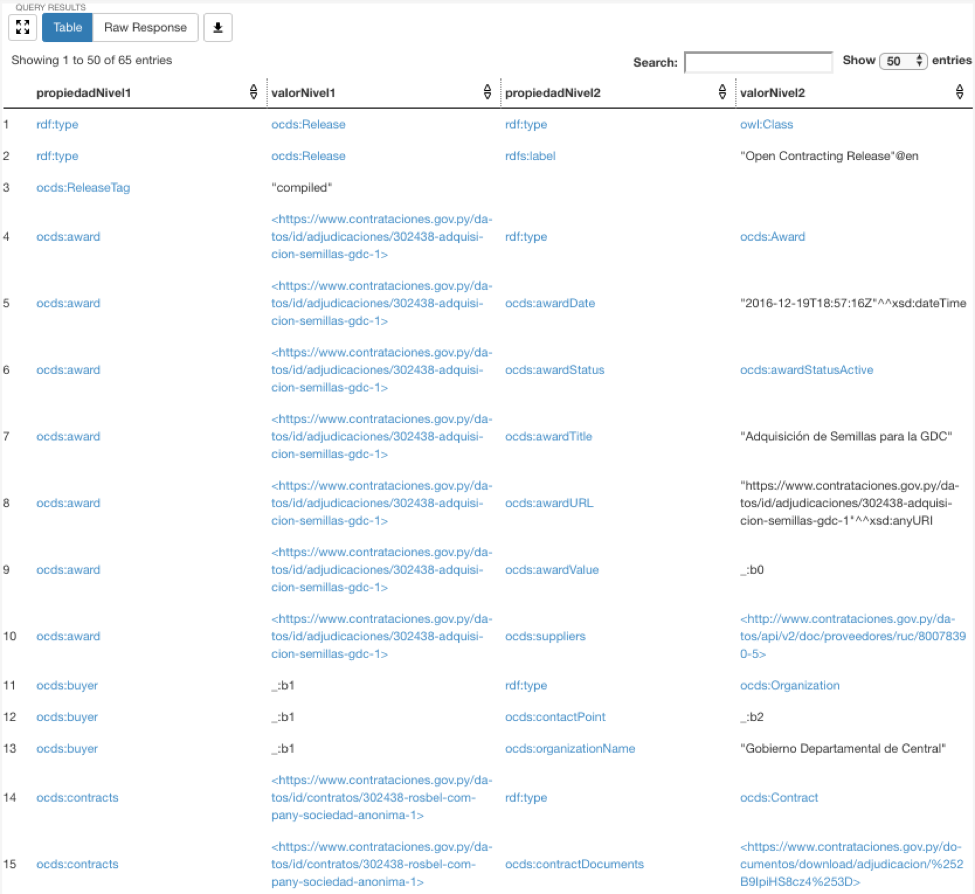
\includegraphics[width=150mm]{figuras/caso1Resultado.png}
    \caption{Despliegue de resultado de la consulta de l caso 1}
    \label{img:caso1Resultado}
 \end{figure}
